\documentclass[10pt,twocolumn,letterpaper]{article}

\usepackage{cvpr}
\usepackage{times}
\usepackage{epsfig}
\usepackage{graphicx}
\usepackage{amsmath}
\usepackage{amssymb}

% Include other packages here, before hyperref.

% If you comment hyperref and then uncomment it, you should delete
% egpaper.aux before re-running latex.  (Or just hit 'q' on the first latex
% run, let it finish, and you should be clear).
\usepackage[breaklinks=true,bookmarks=false]{hyperref}

\cvprfinalcopy{} % *** Uncomment this line for the final submission

\def\cvprPaperID{****} % *** Enter the CVPR Paper ID here
\def\httilde{\mbox{\tt\raisebox{-.5ex}{\symbol{126}}}}

% Pages are numbered in submission mode, and unnumbered in camera-ready
%\ifcvprfinal\pagestyle{empty}\fi
\setcounter{page}{1}
\begin{document}

%%%%%%%%% TITLE
\title{Classic Methods on Color Based Ball Tracking}

\author{Breno Leite\\ Guilherme Leite\\
Instituto de Computa\c{c}\~ao --- UNICAMP\\
}

\maketitle
%\thispagestyle{empty}

%%%%%%%%% ABSTRACT
\begin{abstract}
  Abstract
\end{abstract}

%%%%%%%%% BODY TEXT
\section{Introduction}\label{sec:intro}

Ball tracking is a classical problem present in a diverse range of
applications. Since the early days of robotics where it was used to track
balls in a controlled environment up to today's sports coverage with cluttered
background, occlusion, many players in field and camera's shot with spectators
in the background. To cope with such noisy situations ball tracking nowadays
has to make use of a range of techniques to operate, like training a neural
network to learn and detect a ball at a given frame, use a physics model to
estimate the probable trajectory of the ball or use tiny details such as the
way a player moves when in possession of the ball.

In this work we focus on the classical methods that lead these researches up
to this point today, in Section~\ref{sec:work} we cover some the literature
around the problem, classical and modern approaches to solve the problem, in
Section~\ref{sec:method} we explain our step by step into constructing the
solution, in Section~\ref{sec:result} we cover the experiments performed,
explaining the weakness and strength of the solution for each experiment and
how they were solved in the next one, at last we show how the solution
performs in a real world environment, a Robocup's soccer match and in
Section~\ref{sec:conclusion} are related the importance of implementing this
work and how far this branch of computer vision has come.

%-------------------------------------------------------------------------

\section{Related Work}\label{sec:work}

Ball Tracking has been studied for a long time, in a diverse range of applications.  Some projects  are interested in soccer's ball tracking~\cite{seo1997ball,  tong2004effective, choi2004probabilistic}, others are interested in  volleyball~\cite{chen2007physics} and basketball \cite{ maksai2016players}.   Normally, These works use a wide range of techniques to overcome the problems,  in which motion estimation, Hough circle transform and Kalman filter are included.

In this project the focus is on colored balls, which was very popular in the robot-cup competition~\cite{kitano1997robocup, simon2000robust, kitano1998robocup}.  In order to overcome the problem some usual techniques were studied. Lucas and Kanade motion flow~\cite{tomasi1992shape, tomasi1991detection} was studied in order to reduce total cost of the algorithm.  It predicts the motion flow, which helps the algorithm of detection to be faster and reduce computational cost.

Another technique used in the project is the Hough circle
transform~\cite{illingworth1987adaptive}, which enable  the algorithm to find
circles in the data turning it more robust to noise present in the scene. And
lastly, Kalman filter was studied in order to overcome occlusion problems~\cite{ristic2004beyond}, a vast number of tracking problems use the power of Kalman filter to improve the tracking performance~\cite{satoh2004color}.


%-------------------------------------------------------------------------
\section{Methodology}\label{sec:method}

Initially the tracking was perform only by a color detector, using the color space HSV to select a color range that would create a mask. In this mask every pixel in the range is set to a white color and everything else to black, afterwards two erosion and dilation are applied to reduce noise. In sequence, the connected components are extracted from the resulting mask in order to filter out small areas, the resulting components are possible balls found in the scene. Each of these selected regions has a center of mass, the coordinate of this point is the supposed ball's position in the scene, later on this information will be called ``tracking position''.

After detecting these supposed areas (``balls'') a Hough Circle Transform  is
used, and it tries to fit circles in these areas. The Hough Circle Transform
depends of two parameters passed to the Canny Edge Detector, which is used
inside the Hough algorithm. $param2$ also called accumulator threshold is one of
these parameters, since hough circle transform uses a voting system to better
estimate the center of the circle it has found, this accumulator influences on
how loose the fitting is, lowest values being responsible for false circles
detection.

In the videos a high value ($param2 = 200$) was used to this parameter, and it was decreased while no circles were found. This approach ensures the algorithm to get best circle predictions, but it has a really slow performance. In order to make the system to work on real time, this parameter needs to be set as a small value ($param2 = 80$), which could decrease the precision of the detection. Using Hough Circle Transform the tracking narrows down to track only the roughly rounded shapes in the mask.

Applying the color detection every frame is not efficient, even worse when using
Hough transform to filter the results. In order to overcome this problem the LK
motion flow was implemented, enabling the detection to be applied  in every $N$
frames, which is called re-sampling. There is a trade-off using the LK motion,
a high re-sampling interval means a worse precision of the model, but a better
performance of the solution.

LK motion flow is enough to estimate the ball position, but it always depends on
the last frame. In a scenario in which the ball is occluded for more than a
couple of frames  LK motion will completely lose its estimative. In order to
overcome this problem, Kalman filter is used to predict the ball trajectory
when it is occluded using previous estimatives.

%-------------------------------------------------------------------------
\section{Results}\label{sec:result}

The experiments were designed to stress the effect of each new feature that was incrementally added in the project. A controlled environment was set to perform the experiments, including a blank background, artificial white lighting, fixed camera and three balls of the same size and material, two yellow and one blue.

\subsection{Single color detection}

In this experiment the goal was to precisely track a single ball throughout the camera's view. The Figure \ref{fig:single_color} shows the result of the algorithm implemented.

\begin{figure}[!h]
\centering
\setlength{\fboxsep}{1pt}
\setlength{\fboxrule}{1pt}
\fbox{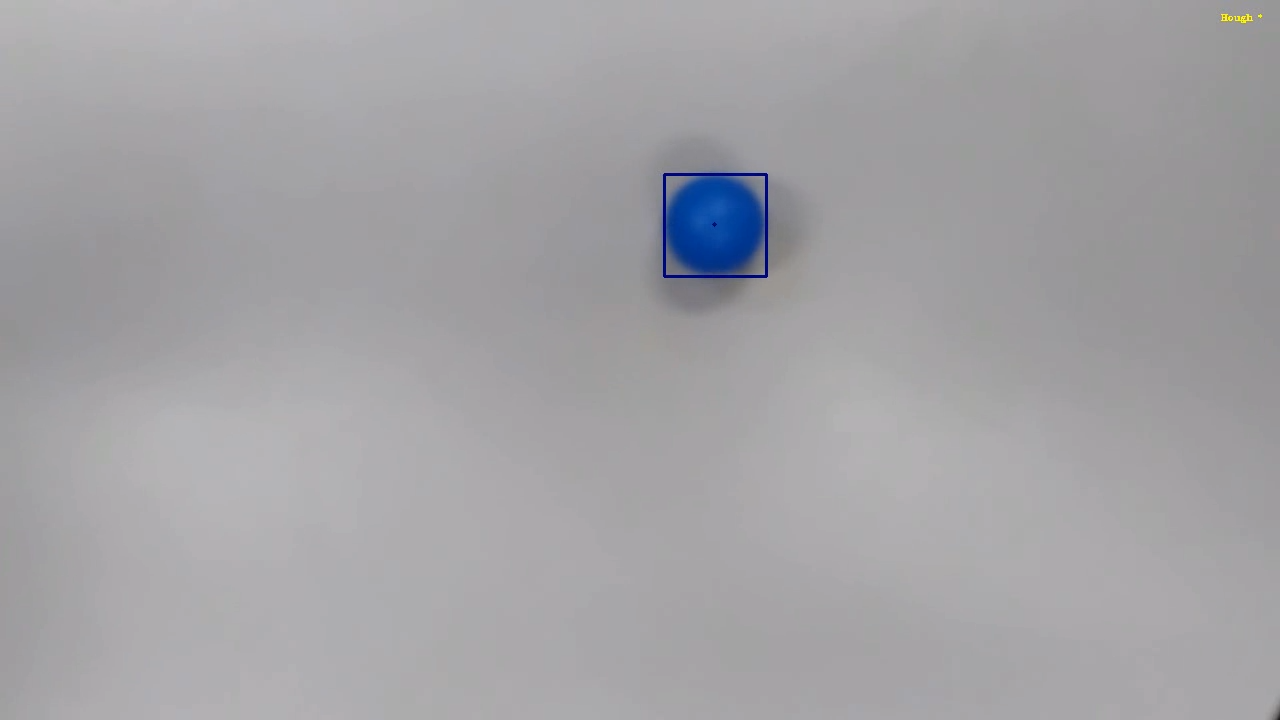
\includegraphics[scale=0.15]{images/single_color}}
\caption{Detection of a colored ball.}\label{fig:single_color}
\end{figure}

The color detection applied to every frame was able to track the ball throughout the camera's view. This solution showed itself insufficient when some objects were introduced, with different shapes other than a sphere but same color as the ball.

\subsection{Two different color tracking}

In this experiment the algorithm has to detect two different balls in the camera's view at the same time, the objective is to show that the algorithm is able to recognize different balls in the same frame.

\subsubsection{Different colors}

In this the object is to detect two different colored balls in the same frame. The Figure \ref{fig:diff_color} shows the result of the detection, in which each ball's  bounding box is shown in different colors.

\begin{figure}[!h]
\centering
\setlength{\fboxsep}{1pt}
\setlength{\fboxrule}{1pt}
\fbox{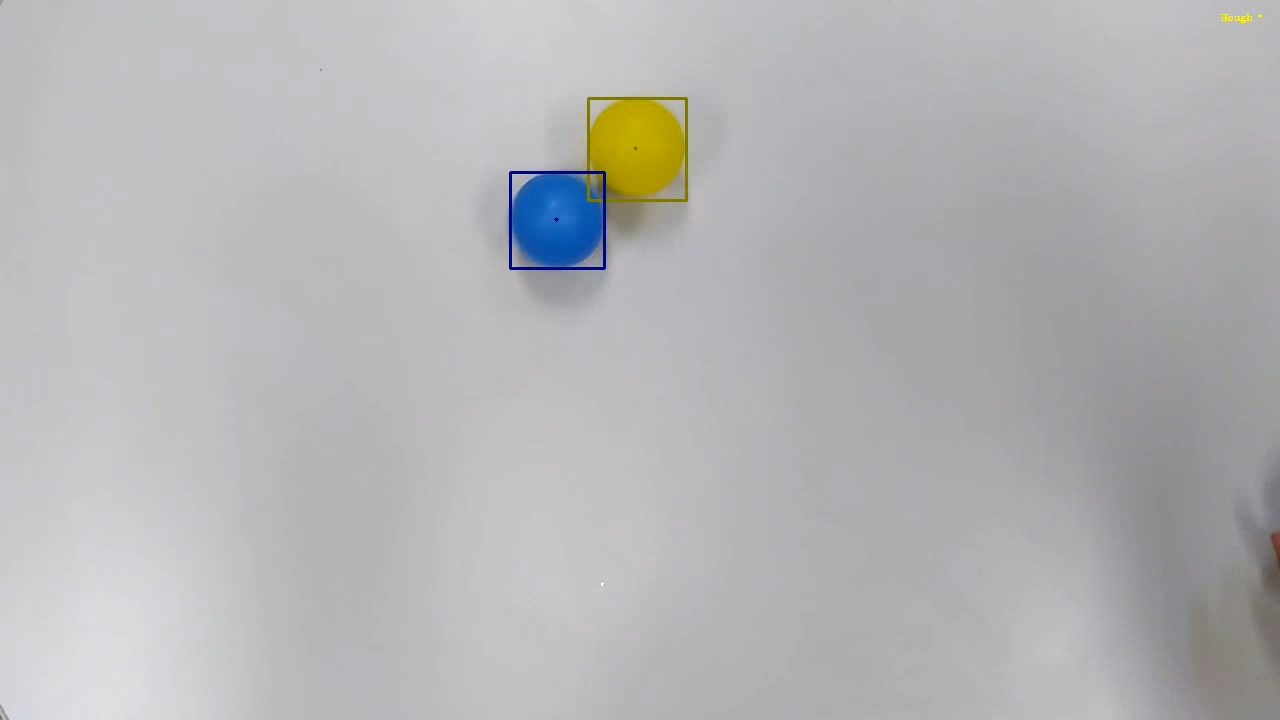
\includegraphics[scale=0.15]{images/diff_color}}
\caption{Detection of two balls with different colors.}\label{fig:diff_color}
\end{figure}

The fine tuning of the colors enabled the solution to isolate one ball from the other, tracking them throughout the camera's view. This limits the solution to be tuned at every application, indoor  and outdoor needs
distinct calibrations.

\subsubsection{Two same color tracking}

In this experiment the objective stills detecting two balls, however they have the same color, which creates a harder problem as the algorithm is relying on colors to detect each one. The results are shown in Figure~\ref{fig:same_color}.

\begin{figure}[!h]
\centering
\setlength{\fboxsep}{1pt}
\setlength{\fboxrule}{1pt}
\fbox{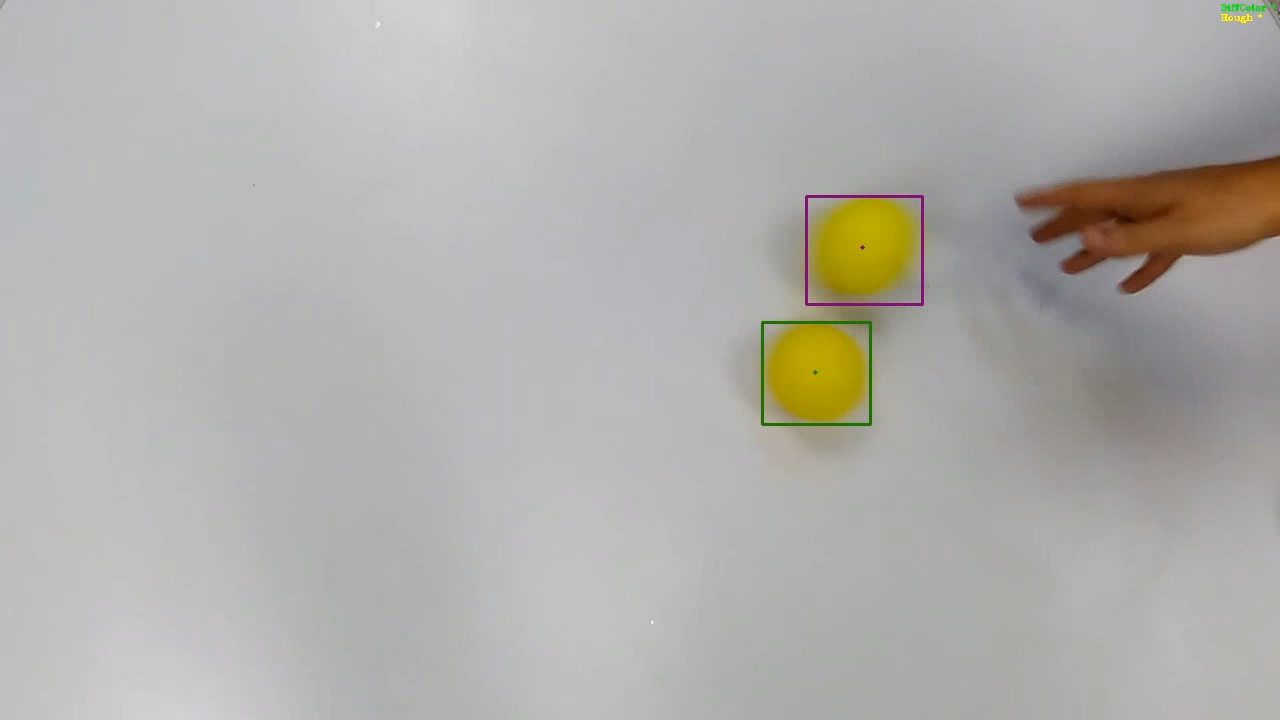
\includegraphics[scale=0.15]{images/same_color}}
\caption{Detection of two balls with the same color.}\label{fig:same_color}
\end{figure}

As seen both balls are detected using different bounding boxes colors, which indicates two different balls. As the algorithm relies on the connected components when both balls are to close it might identify both as just one ball, which is a problem that the proposed architecture could not overcome.

\subsection{Ball tracking alongside with other shapes}

In this experiment a new problem with the color based method is introduced, Figure~\ref{fig:not_hough} shows a confusion made by the detection algorithm.

\begin{figure}[!h]
\centering
\setlength{\fboxsep}{1pt}
\setlength{\fboxrule}{1pt}
\fbox{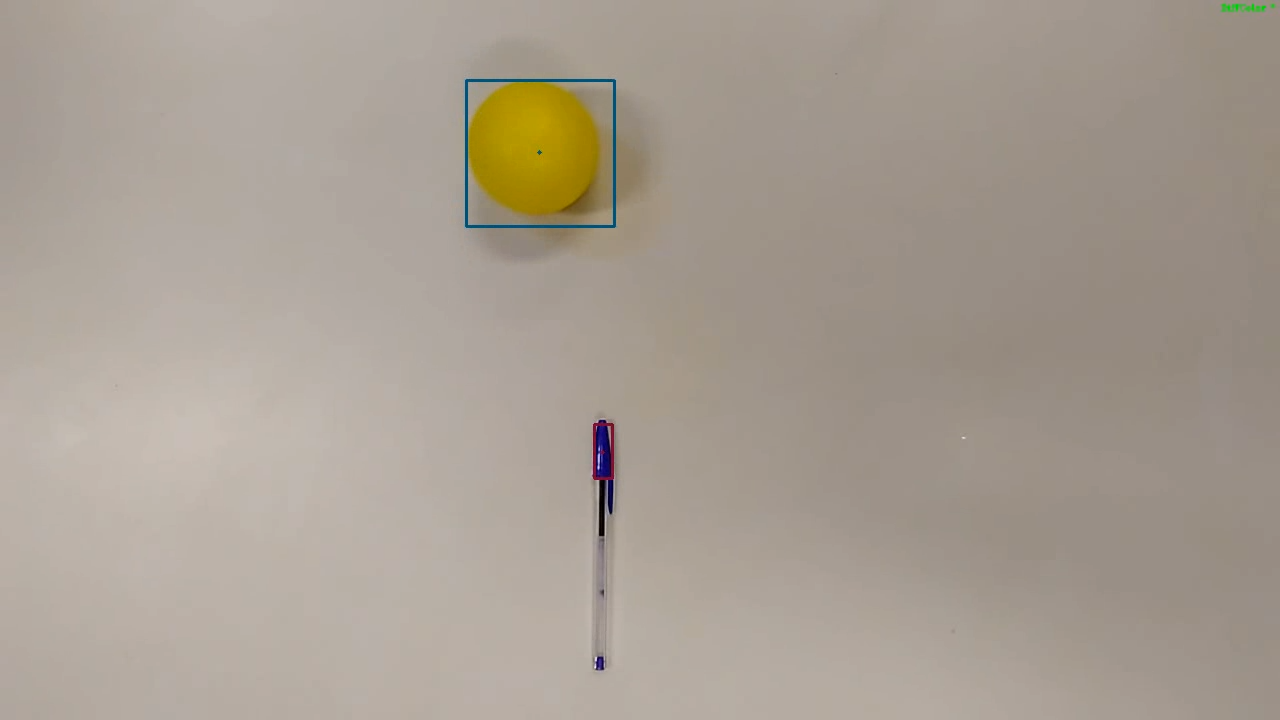
\includegraphics[scale=0.15]{images/not_hough}}
\caption{Detection before the Hough Circle Transform.}\label{fig:not_hough}
\end{figure}

As seen, the solution was not able to differentiate the ball from the pen top. It happens because of the blue color in the pen top, which is considered a blue ball by the mask generated. In order to solve this problem the Hough Circle Transform was used, which filters out the non circle components found in the mask. The results after applying the Hough Transform is shown in Figure~\ref{fig:yes_hough}

\begin{figure}[!h]
\centering
\setlength{\fboxsep}{1pt}
\setlength{\fboxrule}{1pt}
\fbox{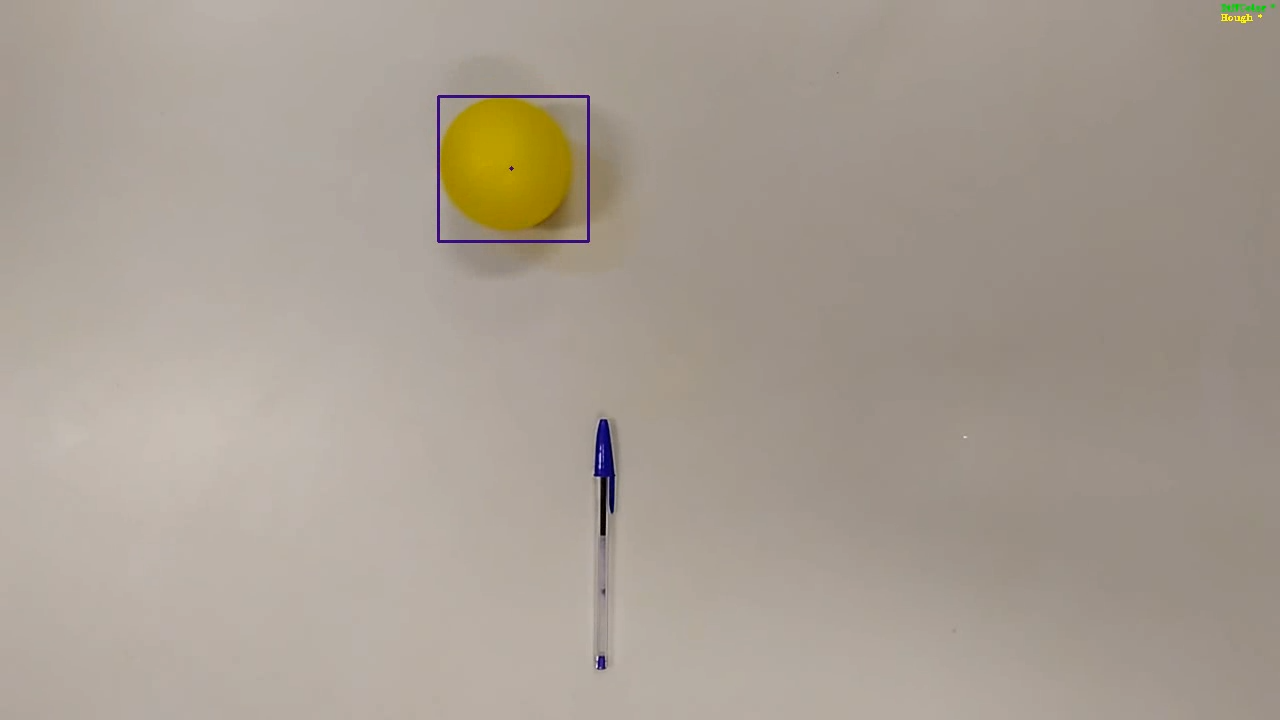
\includegraphics[scale=0.15]{images/yes_hough}}
\caption{Detection after the Hough Circle Transform.}\label{fig:yes_hough}
\end{figure}

In this way,  using the Hough Circle Transform the solution was able to ignore the pen top and track only the ball shaped object.

\subsection{Motion flow tracking compared with color tracking}

Detecting the ball and applying Hough Transform in every frame has a high computational cost, in order to improve the efficiency of the algorithm the Lucas Kanade motion flow was implemented. In this experiment a contrast between the precision and effectiveness is shown. The Figure~\ref{fig:motion_30} shows the motion with a re-sampling of each 5 frames, which increases a little bit the performance of the algorithm. The pink trace indicates the route of the motion, while the blue shows the detection trace made in each frame.

\begin{figure}[!h]
	\centering
	\setlength{\fboxsep}{1pt}
	\setlength{\fboxrule}{1pt}
	\fbox{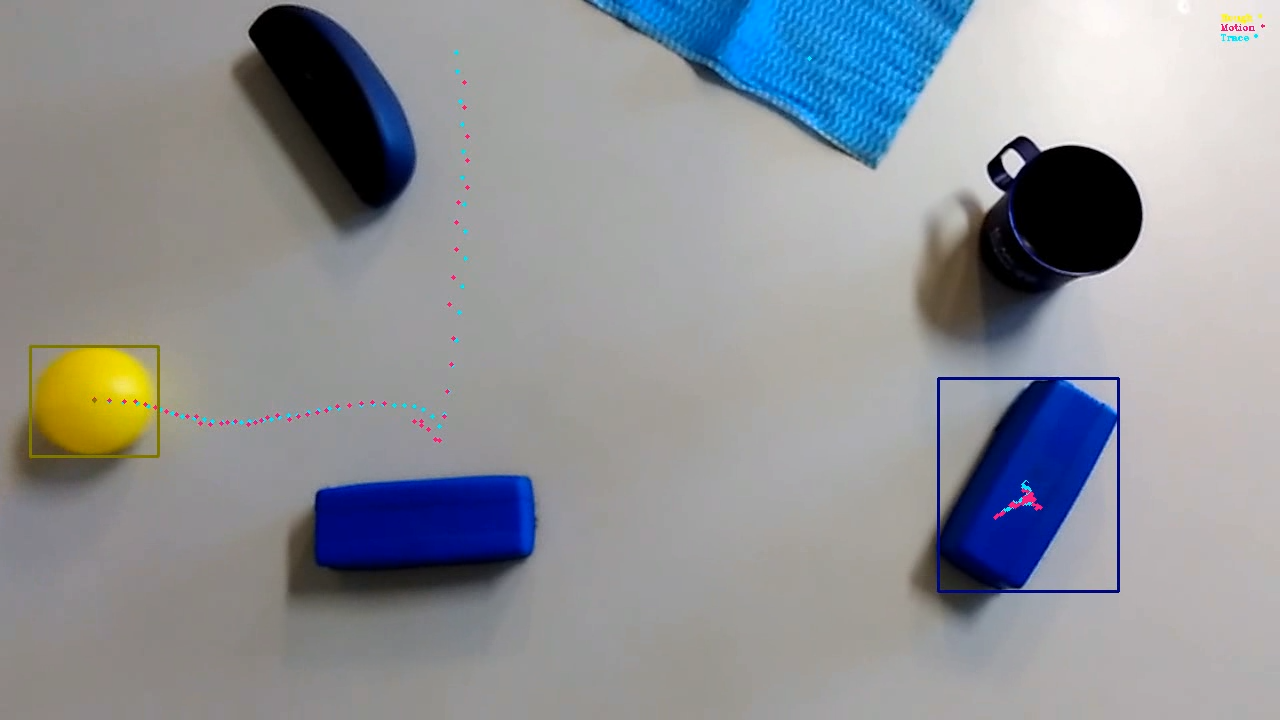
\includegraphics[scale=0.15]{images/motion_5}}
	\caption{Lucas Kanade motion flow applied every 5 frames.}\label{fig:motion_5}
\end{figure}

The results shows a trajectory almost identical, it is noticeable a little lost when the ball hits something, however it is able to recover fast because of the low gap between detections. In contrast, Figure~\ref{fig:motion_30} shows the motion re-sampling in each 30 frames, which increases even more the performance of the algorithm enabling it to become real time in most image sizes.

\begin{figure}[!h]
\centering
\setlength{\fboxsep}{1pt}
\setlength{\fboxrule}{1pt}
\fbox{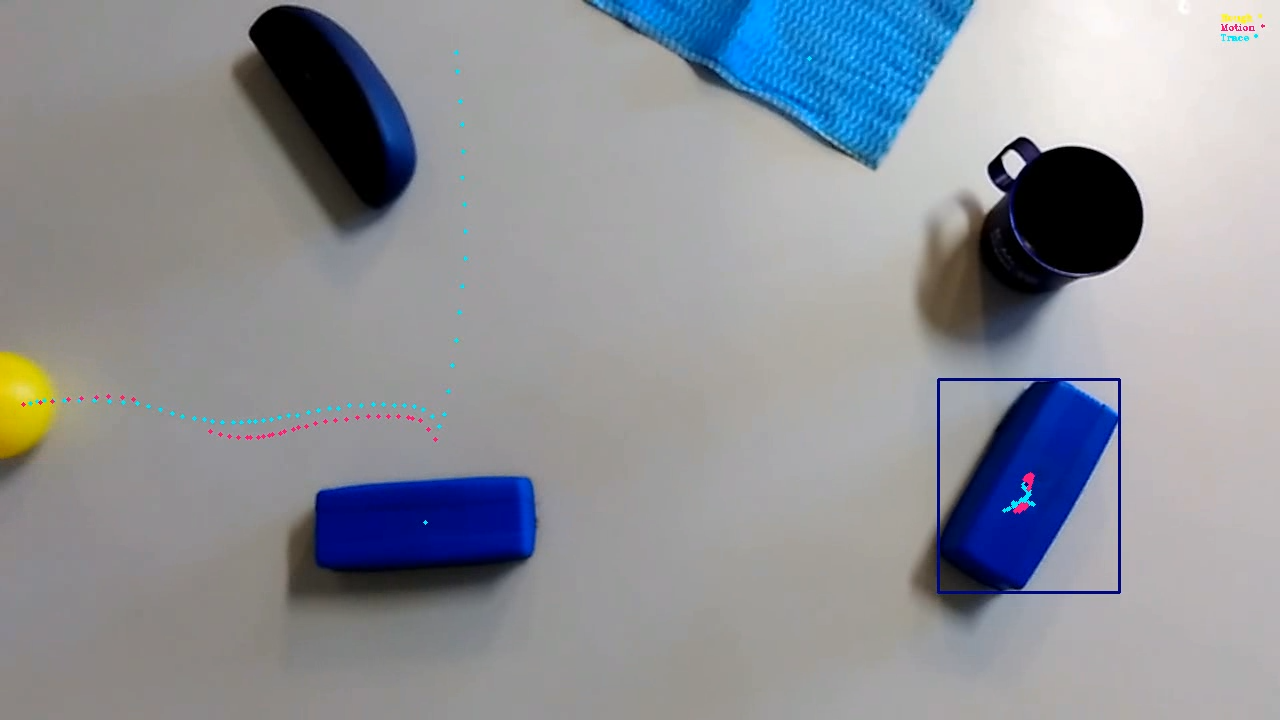
\includegraphics[scale=0.15]{images/motion_30}}
\caption{Lucas Kanade motion flow applied every 30 frames.}\label{fig:motion_30}
\end{figure}

This experiment shows that the motion lose a good amount of frames in the beginning of the video, mainly because the flow takes some time to be detected which is even harder with the re-sampling rate. It is also noticeable that in the ball hits the motion takes more time to correct the position, however it is still a good assumption when comparing the overall performance (precision vs time performance).

\subsection{Occlusion}

In order to check the results of the Kalman filter implemented, a scenario with occlusion is shown in the Figure~\ref{fig:occlusion}. The blue trace is the detection positions, and the orange is the position estimated by the Kalman filter implemented.

\begin{figure}[!h]
\centering
\setlength{\fboxsep}{1pt}
\setlength{\fboxrule}{1pt}
\fbox{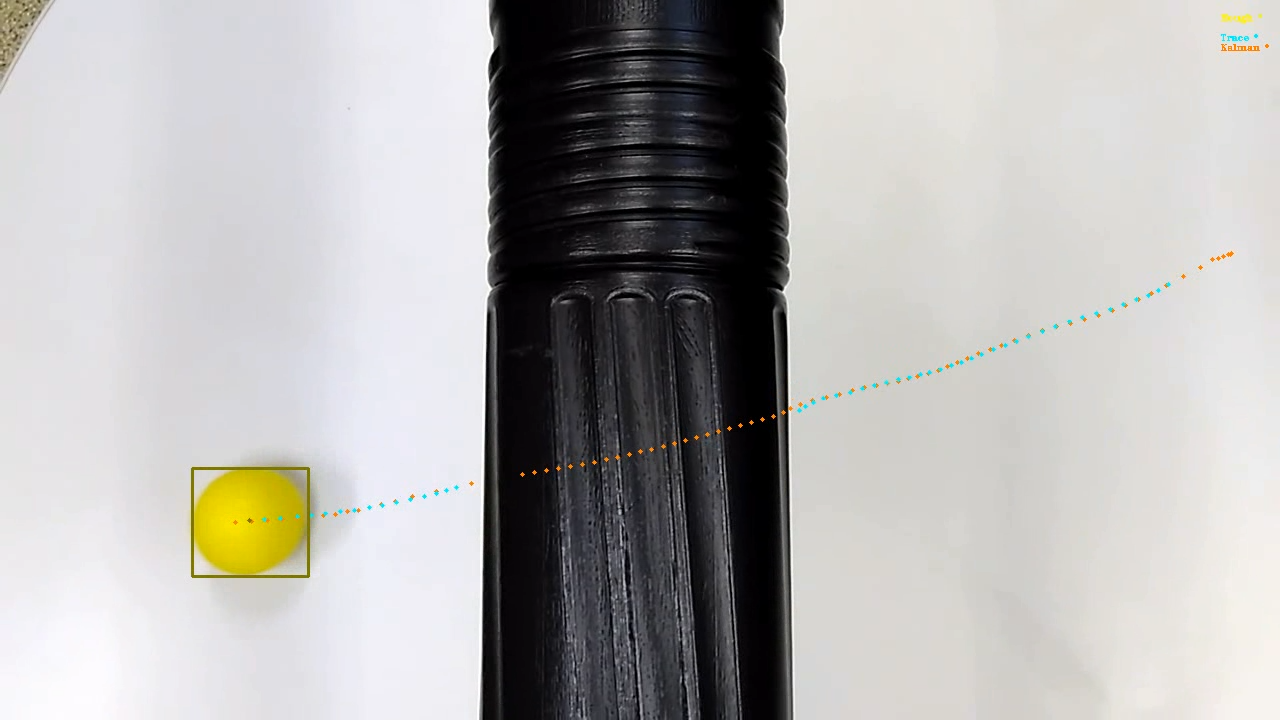
\includegraphics[scale=0.15]{images/occlusion}}
\caption{Kalman filter applied to overcome occlusion.}\label{fig:occlusion}
\end{figure}

As seen, the solution was able to overcome occlusion, since it was able to estimate the ball's trajectory under occlusion. The filter worked best with balls in low speed and couldn't estimate a position if the ball changed directions whilst occluded, as was already expected.

\subsection{Robocup ball tracking}

In this experiment the algorithm was tested under a competition's environment, some adjustments were made in order to tune the color to the orange ball. The Figure~\ref{fig:robocup_1} shows a example of the algorithm working on this scenario.

\begin{figure}[!h]
\centering
\setlength{\fboxsep}{1pt}
\setlength{\fboxrule}{1pt}
\fbox{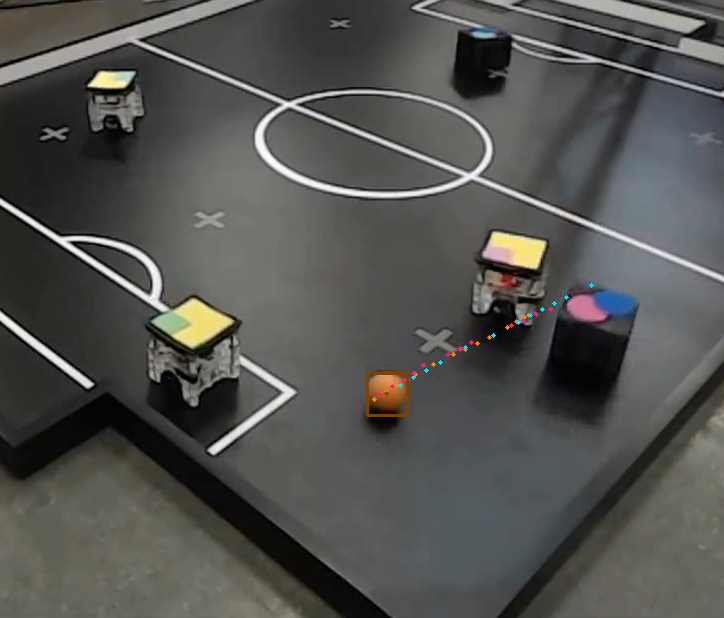
\includegraphics[scale=0.15]{images/robocup_1}}
\caption{All features applied in a Robocup soccer match.}\label{fig:robocup_1}
\end{figure}

As seen, the algorithm was able to detect and predict the ball's position, the motion (pink trace) and the Kalman filter (orange trace) shows good results compared with the detection position trace (blue trace). The LK motion flow obtained a really good result in overall, even when the ball drastically changes direction  the algorithm could rapidly correct the trace.  However,  the Kalman filter easily lost track when the ball drastically changes direction, specially when occluded. The Figure~\ref{fig:robocup2} shows one example that the Kalman filter is lost because of the ball stopping at the wall.

\begin{figure}[!h]
	\centering
	\setlength{\fboxsep}{1pt}
	\setlength{\fboxrule}{1pt}
	\fbox{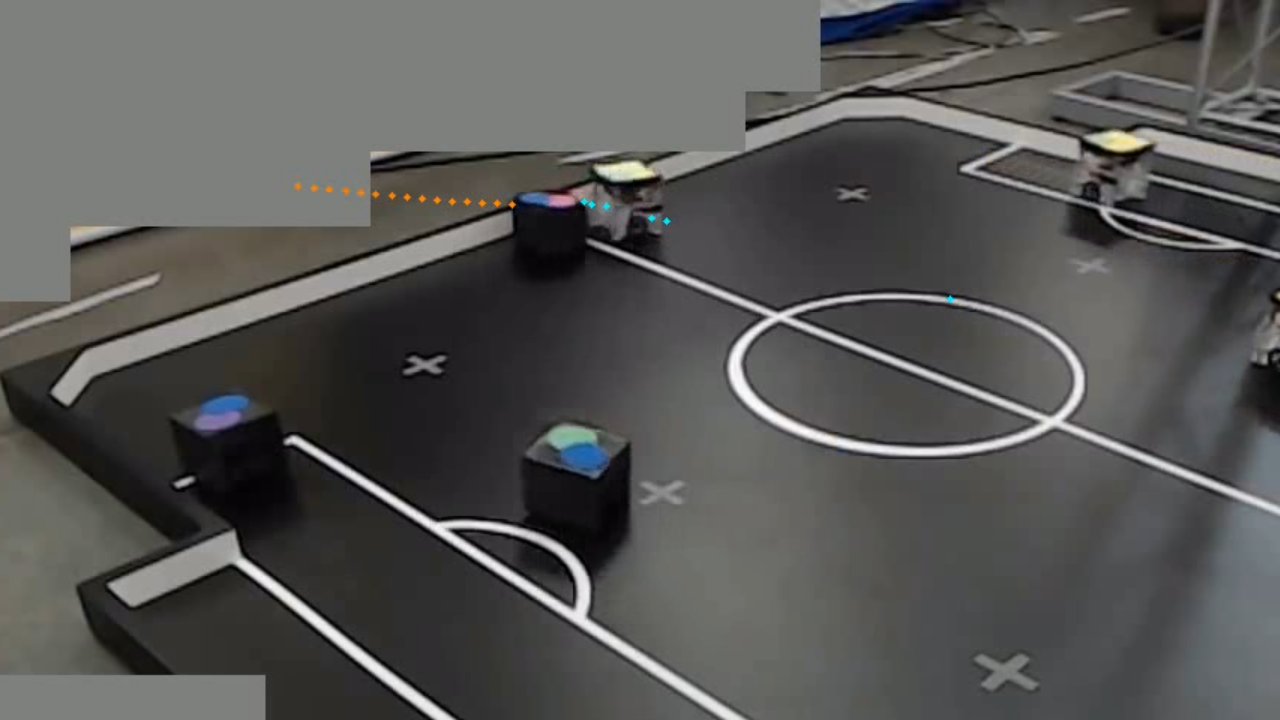
\includegraphics[scale=0.15]{images/robocup_2}}
	\caption{All features applied in a Robocup soccer match.}\label{fig:robocup2}
\end{figure}

%-------------------------------------------------------------------------
\section{Conclusion}\label{sec:conclusion}

As seen the classic methods were able to track and overcome some of the
challenges presented in this project. It could even work good in a real example like the Robocup soccer match, however it is noticeable that the algorithm's precision is worse than in a totally controlled environment.

In harder scenarios, as a soccer, volleyball, and basketball games the algorithm had  bad results, in those scenarios physics models are used to describe the parabolic trajectory of the ball, or even  more complex models, which uses different clues, like the fact that a basketball player handling the ball moves differently from the others.

In this project  many of the course's topics were covered and applied, clearing our sights towards their weakness and strength in each scenario. As future work, the color based detection could be replaced with a deep neural network in order to locate the initial position of the ball. This approach could improve the overall results, and enable the algorithm to deal with harder environments.

{\small
\bibliographystyle{ieee}
\bibliography{egbib}
}

\end{document}
